\documentclass[9pt,twocolumn,twoside]{gsag3jnl}
\usepackage{gensymb}

\articletype{inv} % article type
% use \nameref to refer to cross citations (i,e cite sections in this paper)

\newcommand{\cel}{\emph{C.~elegans}}
\newcommand{\fog}{\emph{fog-2}}
\newcommand{\ecol}{\emph{E.~coli}}

% gene numbers
\newcommand{\fogn}{1,881}
\newcommand{\agen}{5,592}
\newcommand{\interactionn}{1,318}
\newcommand{\coexpressed}{905}
\newcommand{\intersectn}{1,040}

% tf numbers
\newcommand{\tfaging}{145}
\newcommand{\tffog}{60}
\newcommand{\tfinteraction}{36}

% number of genes in gold standard
\newcommand{\goldn}{1056}
\newcommand{\goldfound}{506}
\newcommand{\goldpval}{$<10^{-38}$}

% website commands
\newcommand{\website}{\url{https://wormlabcaltech.github.io/Angeles_And_Leighton_2016/}}
\newcommand{\webref}{\href{https://wormlabcaltech.github.io/Angeles_And_Leighton_2016/}{website}}

\title{\fog{} is a molecular mimicry of early aging in \cel{}}

\author[$\ast$, $\dagger$]{David Angeles-Albores}
\author[$\ast$, $\ddagger$]{Daniel H Leighton}
\author[$\dagger$]{Tiffany Tsou}
\author[$\dagger$]{Tiffany K. Shaw}
\author[$\S$]{Igor Antoshechkin}
\author[$\dagger$, 1]{Paul W Sternberg}

\affil[$\ast$]{Co-First Authors}
\affil[$\dagger$]{Department of Biology and Biological Engineering, and Howard Hughes Medical Institute, Caltech, Pasadena, CA, 91125, USA
}
\affil[$\ddagger$]{Department of Human Genetics, Department of Biological Chemistry, and Howard Hughes Medical Institute, University of California, Los Angeles, Los Angeles, CA 90095, USA.}
\affil[$\S$]{Department of Biology and Biological Engineering, Caltech, Pasadena, CA, 91125, USA}
% \affil[$\ast\ast$]{Department of Biology, Stanford, Stanford, CA, 94305, USA.}

\keywords{\cel{} \\ \fog{} \\ aging \\ transcriptome}

\runningtitle{Effects of Life History on the Transcriptomic Phenotypes of Two  Genotypes of \cel} % For use in the footer

\correspondingauthor{Angeles-Albores}

\begin{abstract}
\end{abstract}

\setboolean{displaycopyright}{true}

\begin{document}

\maketitle{}
\thispagestyle{firststyle}
\logomark{}
\articletypemark{}
\marginmark{}
\firstpagefootnote{}
\correspondingauthoraffiliation{Contact: pws@caltech.edu, Address: Department of Biology and Biological Engineering, and Howard Hughes Medical Institute, Caltech, Pasadena, CA, 91106, USA}
\vspace{-11pt}%


\section{Introduction}
\label{sec:introduction}

% TODO finish
Aging is a natural phenomenon that affects most, if not all, animals.

% TODO middle paragraph
While there has been a long-standing interest in \cel{} longevity and aging past 20 days of life, which has led to a rich literature~\citep{}, there has not been such intense study into the changes that occur during the period of early aging. We refer to early aging as the period of time that occurs between the first day of adulthood (post-L4 molt) and 72 hours later. In this period of time, \cel{} worms undergo a transition between a hermaphroditic, self-fertile stage and its final form as a female worm.

Here, we show that early aging can be divided into two additive components. First, a component that is associated with loss of hermaphroditic sperm and which leads to increases in the levels of transcription factors that are canonically associated with development and cellular differentiation, and enriched in neuronal functions. We also describe a second transcriptomic module consisting of \agen{} genes that is probably associated with biological age in \cel{} and that is invariant between worms that undergo a hermaphroditic egg-laying stage and worms that are never fertilized. Our results can be viewed online in interactive plots at the following address: \website{}/

% figure experiment design
\begin{figure}[htbp]
\renewcommand{\familydefault}{\sfdefault}\normalfont{}
\centering
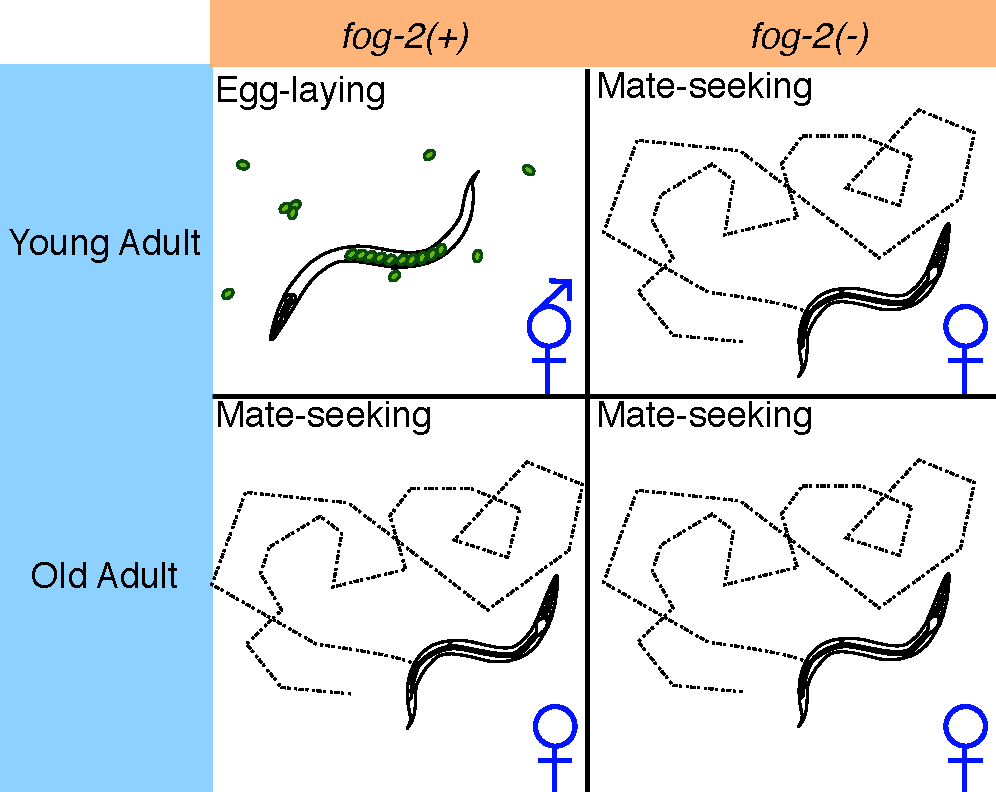
\includegraphics[width=\linewidth]{../output/figs/final_figs/worm_life_fog2_vs_n2.pdf}
\caption{Experimental design to identify genes associated with life-history.
}%
\label{fig:wormlife}
\end{figure}


\section{Materials and Methods}
\label{sec:materials_methods}

\subsection{RNA extraction}
\label{sb:rna_extraction}
Synchronized worms were grown to either young adulthood or the 6th day of adulthood prior to RNA extraction. Synchronization and aging were carried out according to protocols described previously~\citep{}. 1000--5000 worms from each replicate were rinsed into a microcentrifuge tube in S basal (5.85g/L NaCl, 1g/L $\mathrm{K}_2\mathrm{HPO}_4$, 6g/L $\mathrm{KH}_2\mathrm{PO}_4$), and then spun at 14,000rpm for 30s. The supernatant was removed and 1mL of Trizol was added. Worms were lysed by vortexing for 30s at room temperature and then 20 minutes at 4\degree. The Trizol lysate was then spun at 14,000rpm for 10~minutes at 4\degree{} down to allow removal of insoluble materials. Thereafter the Ambion TRIzol protocol was followed to finish the RNA extraction (MAN0001271 Rev. Date: 13 Dec 2012).

\subsection{RNA-seq}
\label{sb:rna_seq}

\subsection{RNA interference}
\label{sb:rnai}
RNAi was performed as described in previous protocols~\citep{}. RNAi bacterial strains were grown in LB plus 100$\mu$g/mL ampicillin overnight. Fresh RNAi cultures were then plated onto NGM agar plates containing 25$\mu$g/mL carbenicillin and 1mM IPTG. N2 or \fog{}\emph{(q71)} hermaphrodites grown on \ecol{} OP50 were bleached onto sterile plates, and starved L1s transferred to recently seeded RNAi plates.
All assays were performed on the offspring of these L1s. Worms grown on every strain were monitored for gross abnormalities, such as sterility, lethality and larval arrest. Control worms in all assays were fed with an anti-GFP RNAi strain. All RNAi worms were grown at 20\degree{} C.

\subsection{Oocyte dropping assay}
\label{sb:oocyte_assay}
We performed a slightly modified oocyte dropping assay based on previously described protocols~\citep{}.~Feminized \fog{}\emph{(q71)} hermaphrodites were picked as virgin L4s the day before the assay to a fresh RNAi plate. The following day, the adult animals were placed on assay plates (NGM agar seeded with 15$\mu$L of \ecol{} OP50 four days earlier), twenty worms per assay, and allowed to incubate at room temperature. Laid oocytes were counted after two hours. Plates were then left at room temperature overnight to serve as lawn-leaving assays.

\subsection{Lawn-leaving assay}
\label{sb:lawn_leaving}
Young adult N2 hermaphrodites were selected the day of the assay and placed on assay plates (same as the oocyte dropping plates), twenty worms per assay, and allowed to incubate at room temperature overnight. Assays for \fog{}\emph{(q71)} hermaphrodites were performed on the same worms as used in the oocyte dropping assays. The following morning, plates were scored for leaving, with any worm touching any part of the bacterial lawn with any part of its body deemed to be “on” the lawn, and all others deemed to be “off”.

\subsection{Brood size counting}
\label{sb:brood_size}
Worms were selected for this assay as L4 hermaphrodites to ensure that all progeny could be counted. For each replicate of each assay, a single worm was placed on a fresh RNAi plate and incubated at 20\degree. Every 1--2 days, the test worm was moved to a fresh RNAi plate, until it stopped laying eggs. Progeny were counted on each plate before they reached adulthood to ensure that only a single generation was counted.

\subsection{Statistical Analysis}
\label{sb:statistics}
\subsubsection{RNA-Seq Analysis.}
RNA-seq alignment was performed using Kallisto~\citep{} with 200 bootstraps. The commands used for read-alignment are in file % TODO
. Differential expression analysis was performed using Sleuth~\citep{}. The following Generalized Linear Model (GLM) was fit:

\begin{equation}
  \log(y_i) = \beta_{0,i} + \beta_{G,i}\dot~G + \beta_{A,i}\dot~A + \beta_{A::G,i}\dot~A~G,
  \label{eqn:GLM}
\end{equation}

where $y_i$ are the TPM counts for the ith gene; $\beta_{0,i}$ is the intercept for the ith gene, and $\beta_{X,i}$ is the regression coefficient for variable $X$ for the $i$th gene; $A$ is a binary age variable indicating young adult (0) or old adult (1) and $G$ is the genotype variable indicating wild-type (0) or \fog{} (1); $\beta_{A::G, i}$ refers to the regression coefficient accounting for the interaction between the age and genotype variables in the $i$th gene. Genes were called significant if the FDR-adjusted q-value for any regression coefficient was less than 0.1. Our script for differential analysis is available on GitHub.

Regression coefficients and TPM counts were processed using Python. Data analysis was performed using the Pandas, NumPy and SciPy libraries~\citep{}. Graphics were created using the Matplotlib and Seaborn libraries~\citep{}.

Tissue Enrichment Analysis was performed using WormBase's TEA tool~\citep{}. We also used the tissue annotation dictionary provided by WormBase to identify genes that were altered in specific tissues.
\subsubsection{Brood Size Analysis.}

Brood size results were analyzed using Welch's t-test to identify genes that were significantly different from a GFP RNAi control. RNAi control results were pooled over multiple days because we could not detect systematic day-day variation. We did not apply FDR or Bonferroni correction because, at a p-value threshold for significance of 0.05, we expected 1 false positive on average per screen.
\subsubsection{lawn-leaving Analysis.}

lawn-leaving results were analyzed using a $\chi^2$ test for categorical variables. Results were considered statistically significant if $p<0.05$. No FDR or Bonferroni correction was applied because the size of the screen was too small, with 1 false positive expected on average per screen. However, the lawn-leaving results suffered from high variance, which can lead to false positive results.
To safeguard against false positive discovery, we used a non-parametric bootstrap to estimate the true $\chi^2$ value. Using a bootstrap does not lead to statistical acceptance of any gene that was not accepted without a bootstrap; however, applying a boostrap does lead to statistical rejection of a large number of results.
\subsubsection{Oocyte Dropping Analysis.}

Oocyte dropping results were analyzed using a non-parametric bootstrapped Mann-Whitney U-test because the GFP control variance was very large relative to the variance of the RNAi treatments. Results were considered statistically significant if $p<0.05$.



\subsection{Data Availability}
\label{sb:data_availability}
Strains are available upon request. File S1 XXXX. File S2 contains XXXX. File S3 contains XXXX. Sequence data are available at GenBank and the accession numbers are listed in File S3. Gene expression data are available at GEO with the accession number: XXXXXX. Code used to generate the simulated data is provided in file XXXX.

\section{Results}
\label{sec:results}
% figure (aging transcriptomics)
\begin{figure}[htbp]
\renewcommand{\familydefault}{\sfdefault}\normalfont{}
\centering
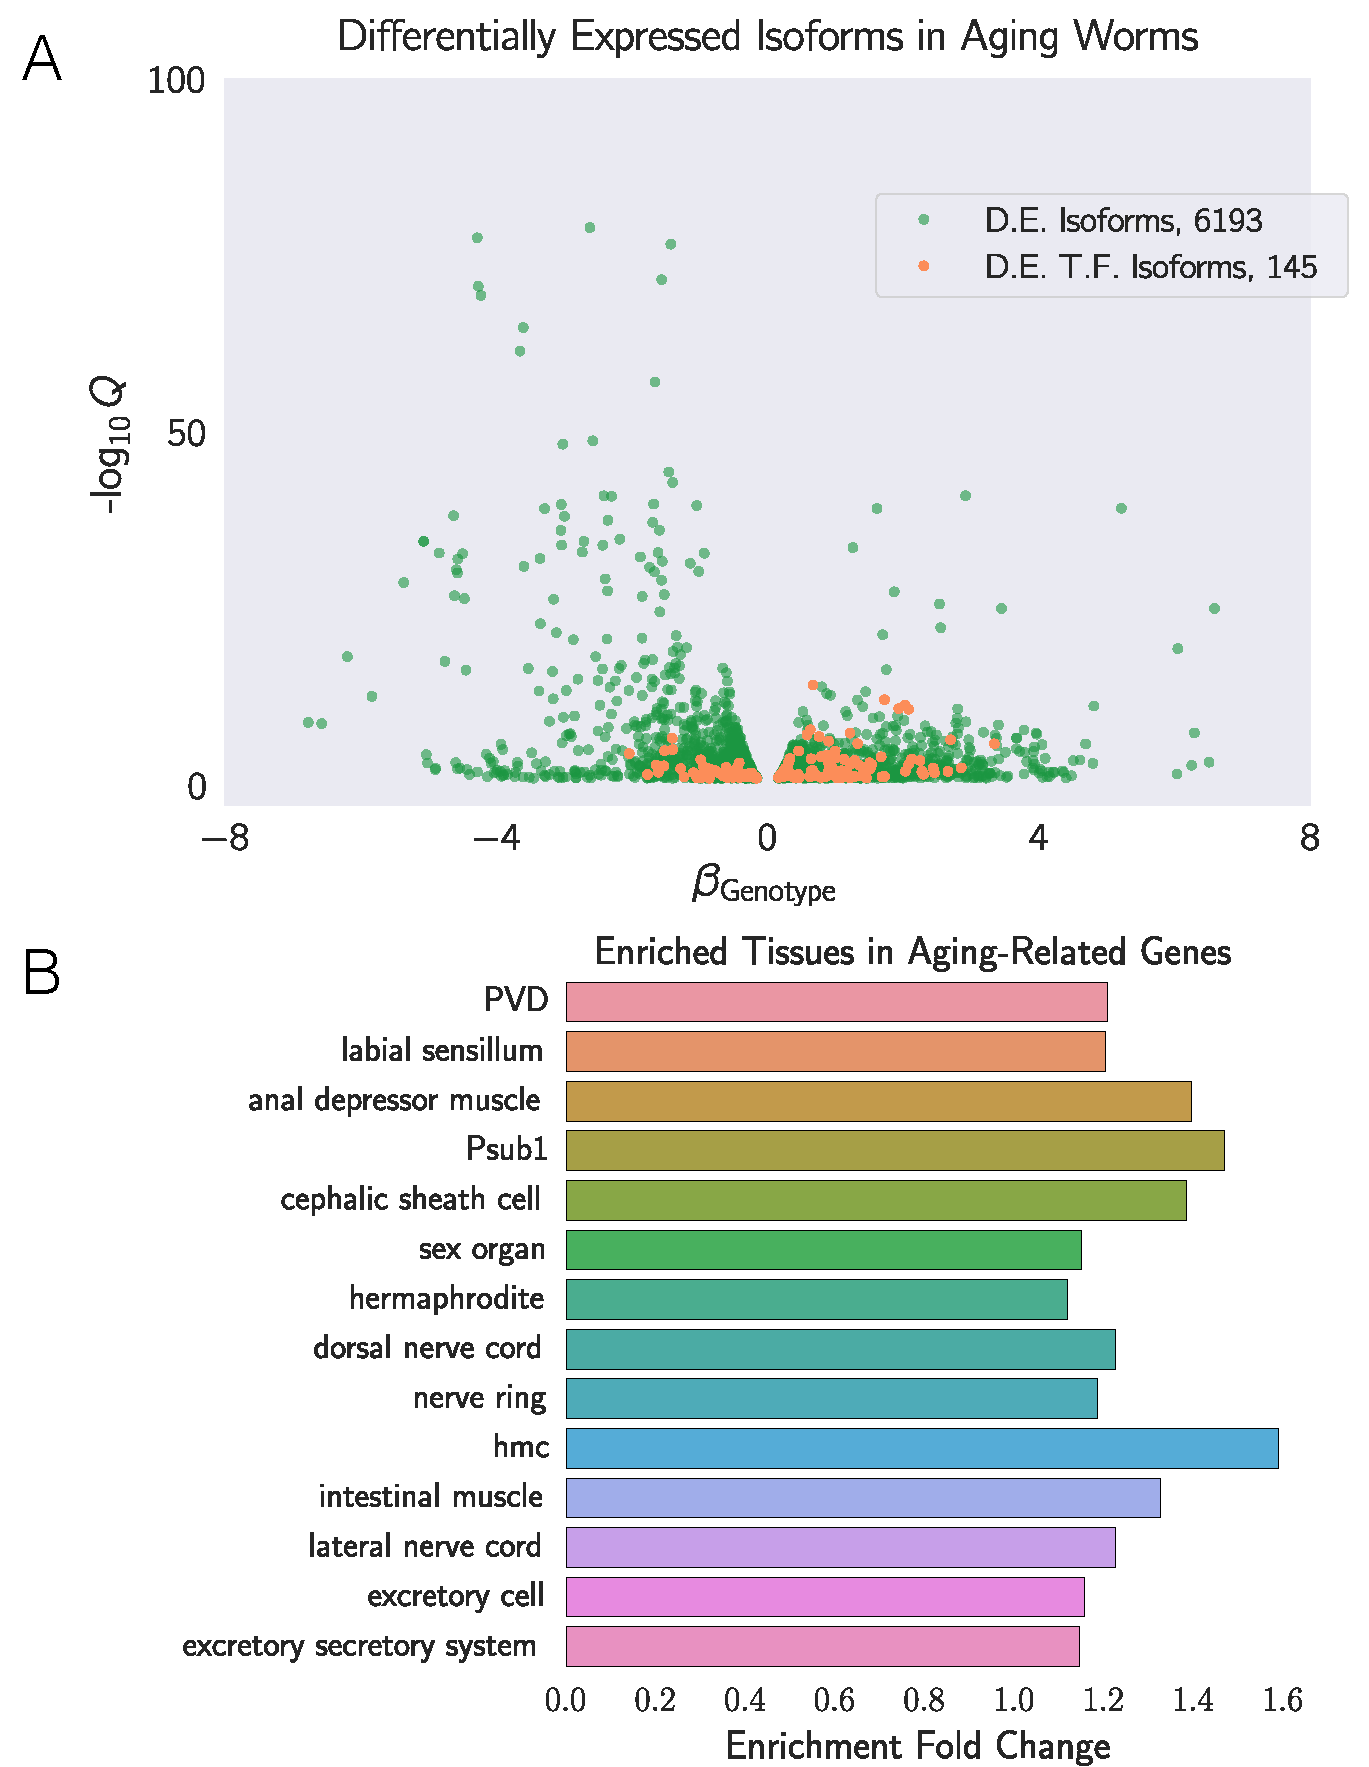
\includegraphics[width=\linewidth]{../output/figs/final_figs/aging_transcriptomics.pdf}
\caption{\textbf{ a} We identified a common aging transcriptome between N2 and \fog{} animals, which showed \agen{}  altered genes. The volcano plot was randomly down-sampled 30\%. \textbf{b} Tissue Enrichment Analysis showed that genes associated with muscle tissues and hypodermis are enriched in this dataset. An interactive version of this graph can be found on our \webref{}.
}%
\label{fig:agingtranscriptome}
\end{figure}

\subsection*{Transcriptomics}
\label{sub:Transcriptomics}

We used a linear generalized model (see \nameref{sb:statistics}) with interactions to identify a transcriptomic profile associated with the \fog{} genotype, a transcriptomic profile of \cel{} aging common to both genotypes. We identified an aging transcriptomic phenotypic consisting of \agen{} genes that were differentially expressed in 6 day old animals relative to 3 day old animals. This constitutes almost one quarter of the genes in \cel{}. Tissue Enrichment Analysis (TEA) showed that muscle-associated and hypodermis-associated genes are particularly enriched in this dataset (see Figure~\ref{fig:agingtranscriptome}).

To verify the quality of our dataset, we generated a list of genes expected to be altered in 6 day old worms using previous literature reports including downstream genes of \emph{daf-12}, \emph{daf-16}, and aging and lifespan extension datasets~\citep{}. Out of \goldn{} genes in our golden standards, we found \goldfound{}. This results was statistically significant with a p-value \goldpval{}.

\begin{table*}[htbp]
\renewcommand{\familydefault}{\sfdefault}\normalfont{}
\centering
\caption{\textbf{Transcription Factor TEA Results.} We ran TEA on the transcription factors associated with aging. Raw results showed a large list of terms associated with embryonic tissues that are neuronal precursors (AB lineage), so we trimmed the results by removing any terms that were expected to show up less than once in our list (if a term is expected to show up $10^{-3}$ times in a list, 1 occurrence is enough to show enrichment in this list). The best 4 results by Q-value are shown below.}
\begin{tableminipage}{\textwidth}
\begin{tabularx}{\textwidth}{XXXX}
\toprule
\header{}Tissue & Expected & Observed & Q-value \\
\bottomrule{}
P11	& 1 & 9 & 0.000006\\
ventral nerve cord &	9 &	26 &	0.000006\\
dorsal nerve cord &	5 &	19 & 0.000006\\
head muscle	& 3	& 13 &	0.000040\\
P7.p & 1 &	6	& 0.001382\\
\bottomrule{}
\end{tabularx}
\label{tab:tea_tf_age}
\end{tableminipage}
\end{table*}

To better understand this dataset, we extracted all the transcription factors that were altered in the aging gene-set. We found \tfaging{} transcription factors. We expected these transcription factors to reflect the same tissue enrichment as the bulk dataset, but the results showed enrichment of hypodermic tissues and neuronal tissues, not muscle (see Table~\ref{tab:tea_tf_age}). Many of these transcription factors have been typically associated with developmental processess, and it is unclear why they would change expression in adult animals. Interactive volcano plots for each gene-set can be found in our \webref{}, where all the transcription factors are shown as green and all significantly altered genes are plotted in gray (no downsampling).

Next, we extracted the regression coefficients associated with genotype change, we were also able to identify \fogn{} genes associated with the \fog{} genotype, including \tffog{} transcription factors. Gonad-related tissues were enriched in this gene set, consistent with the function of \fog{} as a sperm transcription factor. As before, tissue enrichment analysis of these transcription factors reveals that they are involved in neural development. Of the \fogn{} genes that we identified in the \fog{} transcriptome, \intersectn{} genes were also identified in our aging set. Moreover, of these \intersectn{}  genes, \coexpressed{} genes changed in the same direction in age and genotype.

We were surprised at the large fraction of genes that overlapped between these two categories. We built our model to explicitly avoid overlap between variables. Our original expectation had been that certain genes would show a common aging phenotype regardless of genotype; that \fog{} would exhibit a specific set of changes; and that a small set of genes would be altered between genotypes throughout the course of aging. However, the large fraction of genes that exhibit shared changes between both variables suggests that almost all genes that are involved in sperm loss through mutation of \fog{} have an aberrant aging behaviour.

This aberrant behaviour can be most clearly observed by plotting the $\beta$ regression coefficients for each variable against each other. Doing so reveals a clear trend along the line $y=x$. However, our model is built to specifically disallow this. The only situation in which $\beta_\mathrm{aging} = \beta_\mathrm{genotype}$ is a valid statement in our model is when $\beta_\mathrm{aging::genotype} \neq 0$. Therefore, we also plotted $\beta_\mathrm{aging::genotype}$ against $\beta_\mathrm{aging}$. This revealed a strong inverse relationship: The interaction term cancels the aging (or genotype) term. An old, \fog{} worm would be represented as
$\beta_\mathrm{aging} +\beta_\mathrm{genotype} + \beta_\mathrm{aging::genotype} = \beta_\mathrm{genotype}$.
Therefore, genes that are associated with sperm loss through mutation in the \fog{} gene do not change through early aging in these animals. However, in animals that are wild-type, these same genes will eventually change to the same levels as in the \fog{} mutants. In other words, \fog{} partially phenocopies the aging process in wild-type animals 3 days post-adulthood.

% aberrant aging
\begin{figure}[htbp]
\renewcommand{\familydefault}{\sfdefault}\normalfont{}
\centering
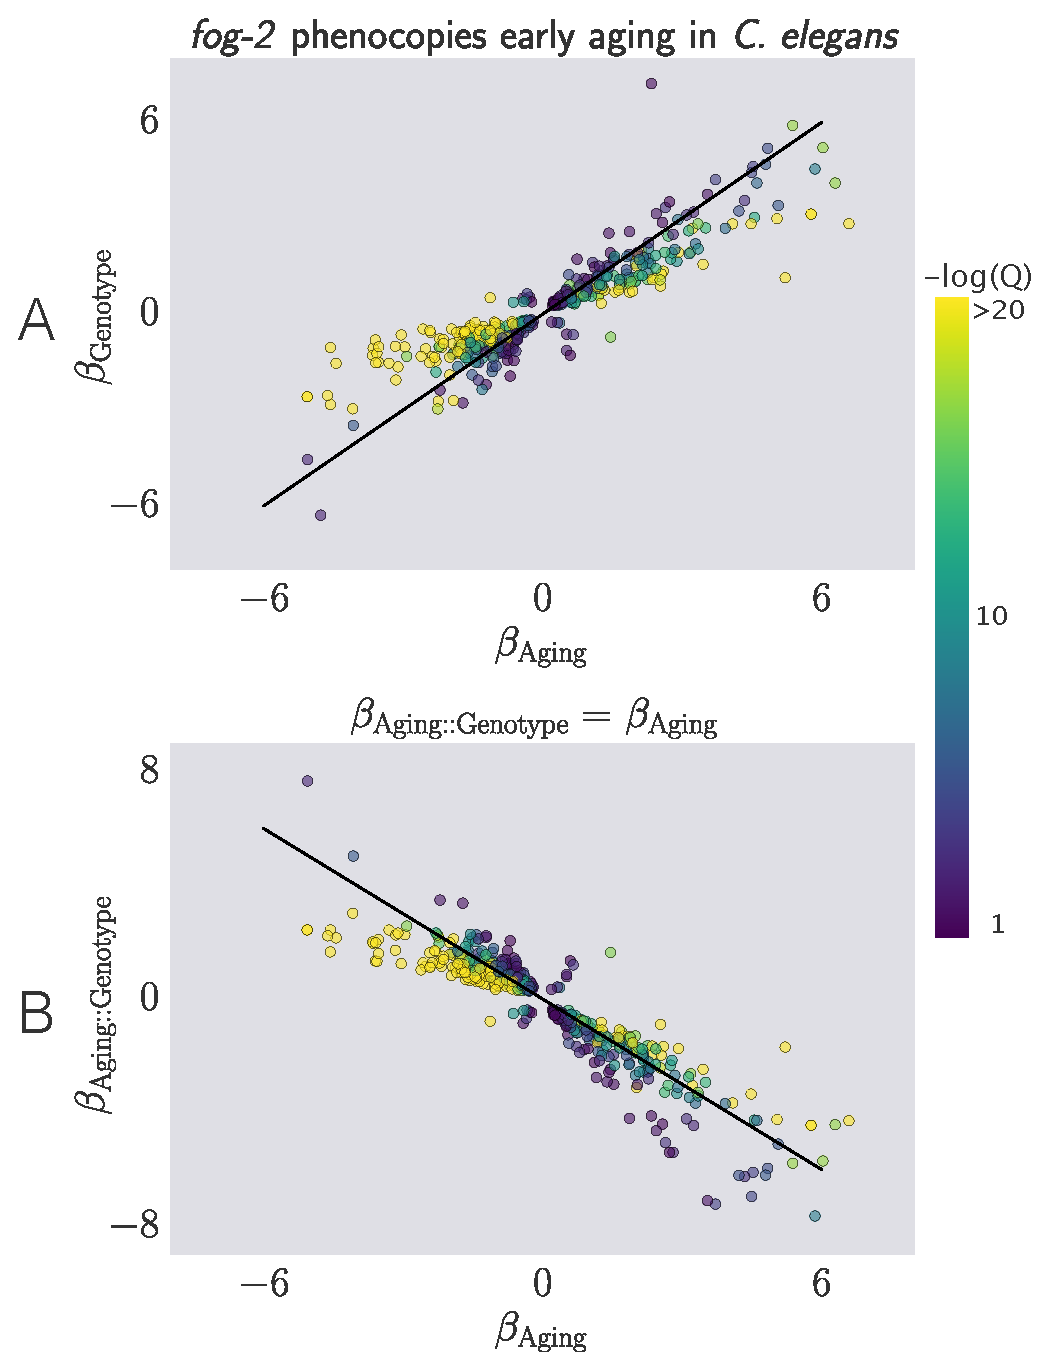
\includegraphics[width=\linewidth]{../output/figs/final_figs/aberrant_aging.pdf}
\caption{ \fog{} partially phenocopies early aging in \cel{}. Feminization by loss of \fog{} is associated with a transcriptomic phenotype involving \fogn{} genes. These genes are also altered in wild-type worms as they progress from young adulthood to old adulthood. However, progression from young to old adulthood in a \fog{} background results in no change in the expression level of these genes. \textbf{a} $\beta_\mathrm{aging}$ vs $\beta_\mathrm{genotype}$ shows that these values have a correlation close to unity. Black line is the line $y=x$, not a line of best fit. \textbf{b} $beta_\mathrm{aging::genotype}$ vs $\beta_\mathrm{aging}$ shows that there is an inverse correlation between these two variables, which means that whereas in a wild-type animal these genes would change expression level as it ages, in a \fog{} animal these genes would not change.
The black line is the line $y=-x$, and is not a line of best fit. For both graphs, color is proportional to $-\log{Q}$. Purple shows Q-values close to 0.1, whereas yellow shows values $<10^{-20}$.
An interactive version of these graphs can be found on our \webref{}.
}%
\label{fig:aberrant_aging}
\end{figure}


\subsection*{Screens}
\label{subs:Screens}

We designed three screens to test our gene sets. We selected gene targets by identifying genes that belonged exclusively to one of the three sets defined previously. We selected two assays that could be performed to test genes associated with genotype change. We reasoned that genes that are negatively correlated with the \fog{} genotype could be associated with fertility, whereas genes that are positively correlated with the \fog{} genotype could be associated with ovulation rate. Moreover, lawn leaving is known to be associated with sperm status~\citep{}, so we decided to perform a second screen to study lawn-leaving behaviour.

% figure 3 (brood assay)
\begin{figure}[htbp]
\renewcommand{\familydefault}{\sfdefault}\normalfont{}
\centering
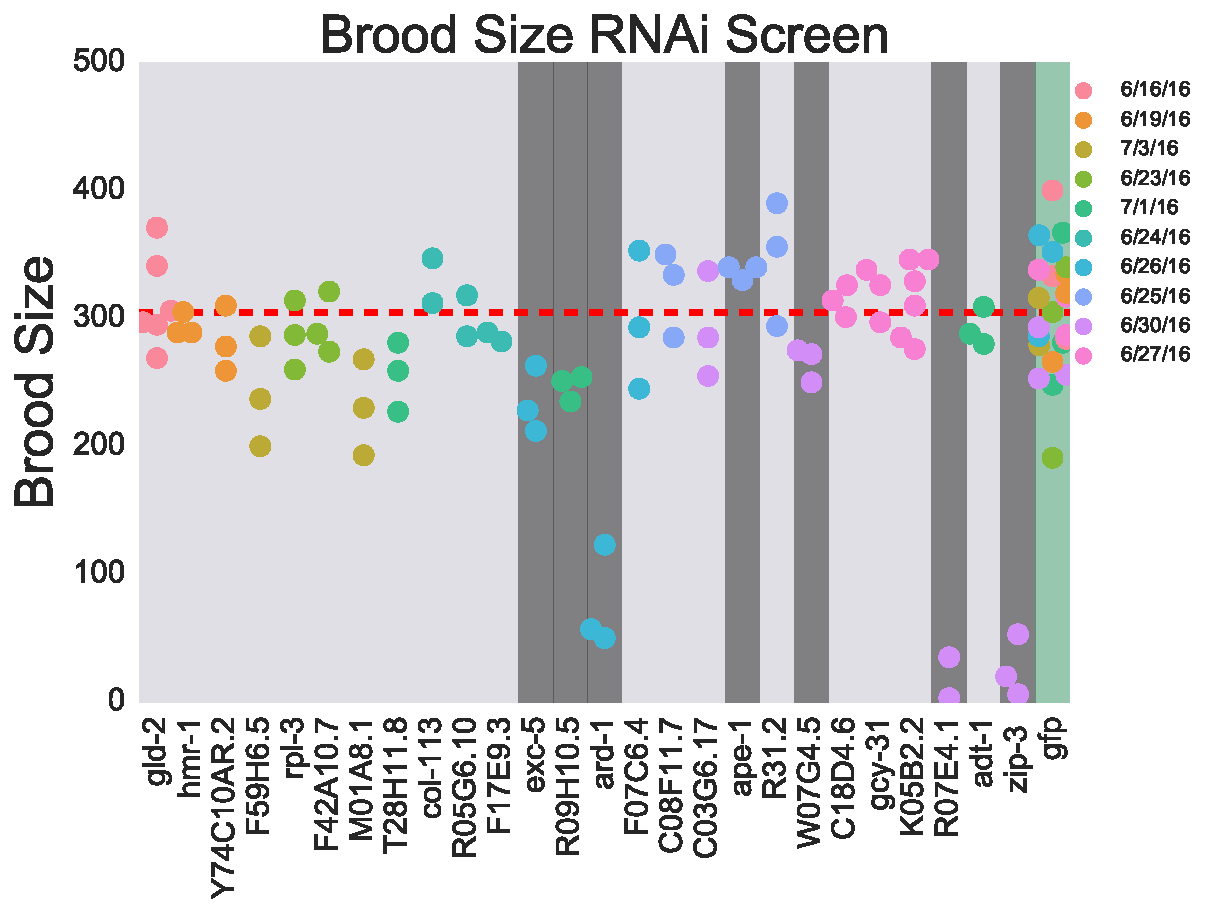
\includegraphics[width=\linewidth]{../output/figs/final_figs/rnai_brood_assay_results.pdf}
\caption{Brood size screen results. GFP control RNAi is shaded in green. Results that are statistically significantly different from GFP are shaded in dark grey. Dotted red line shows the mean of the pooled GFP controls. Points are colored by the date the assay was started on.
}%
\label{fig:broodassay}
\end{figure}

We performed a brood size screen, selecting as targets genes that were upregulated in N2 but downregulated in \fog{}, and we also included some genes from alternative categories if we visually noticed serious decreases in brood size. We identified 9 genes that altered brood size (see Figure~\ref{fig:broodassay}). Of these 7 genes, XXX were previously known. XXX/7 were genes that were associated specifically with the \fog{} phenotype. XXX/7 were associated with aging or life history.

% brood assay
% exc-5
% R09H10.5 - expressed in intestine
% ard-1 - alcohol dehydrogenase, fat content
% ape-1 - p53 deydrogenase, sterile
% W07G4.5 - intestine
% R07E4.1
% zip-3

% figure 5 (oocyte dropping)
\begin{figure}[htbp]
\renewcommand{\familydefault}{\sfdefault}\normalfont{}
\centering
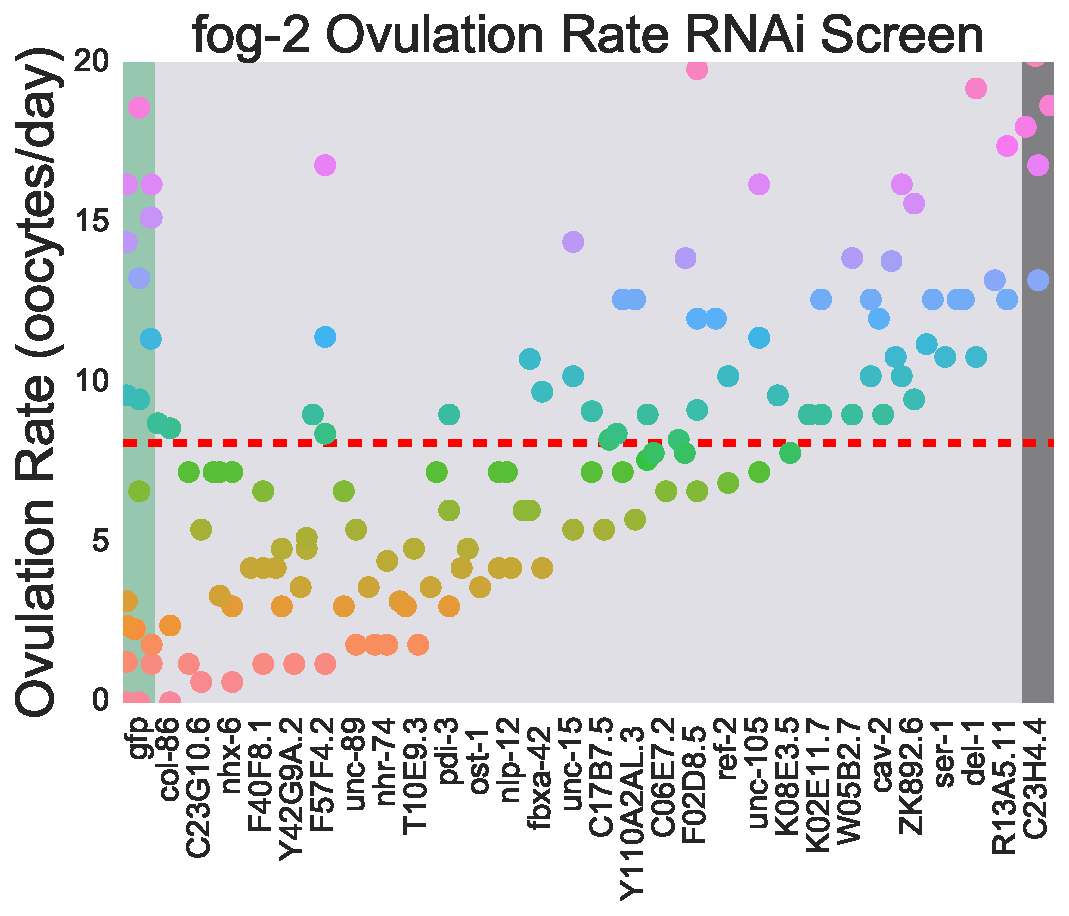
\includegraphics[width=\linewidth]{../output/figs/final_figs/oocyte_rate_assay.pdf}
\caption{Ovulation Rate Assay. GFP control RNAi is shaded in green. Results that are statistically significantly different from GFP are shaded in dark grey. Dotted red line shows the mean of the pooled GFP controls. Points are colored proportionally to their y-coordinate
}%
\label{fig:oocytedropping}
\end{figure}

We reasoned that some of the genes in our genotype dataset might also be associated with ovulation rate in \fog{}. We selected genes that showed upregulation in \fog{} animals and placed them on a lawn for two hours. We observed large variation in the ovulation rate for the control RNAi, and as a result no genes were associated with alterations in ovulation rate. However, the pooled variance across the screen was very similar to the control variance, suggesting that our failure to identify genes was not a result of poor conditions or experimental variance. Our screen identified a single hit: C23H4.4, a carboxyl ester lipase with unknown function.

% figure 4 (lawn-leaving)
\begin{figure}[htbp]
\renewcommand{\familydefault}{\sfdefault}\normalfont{}
\centering
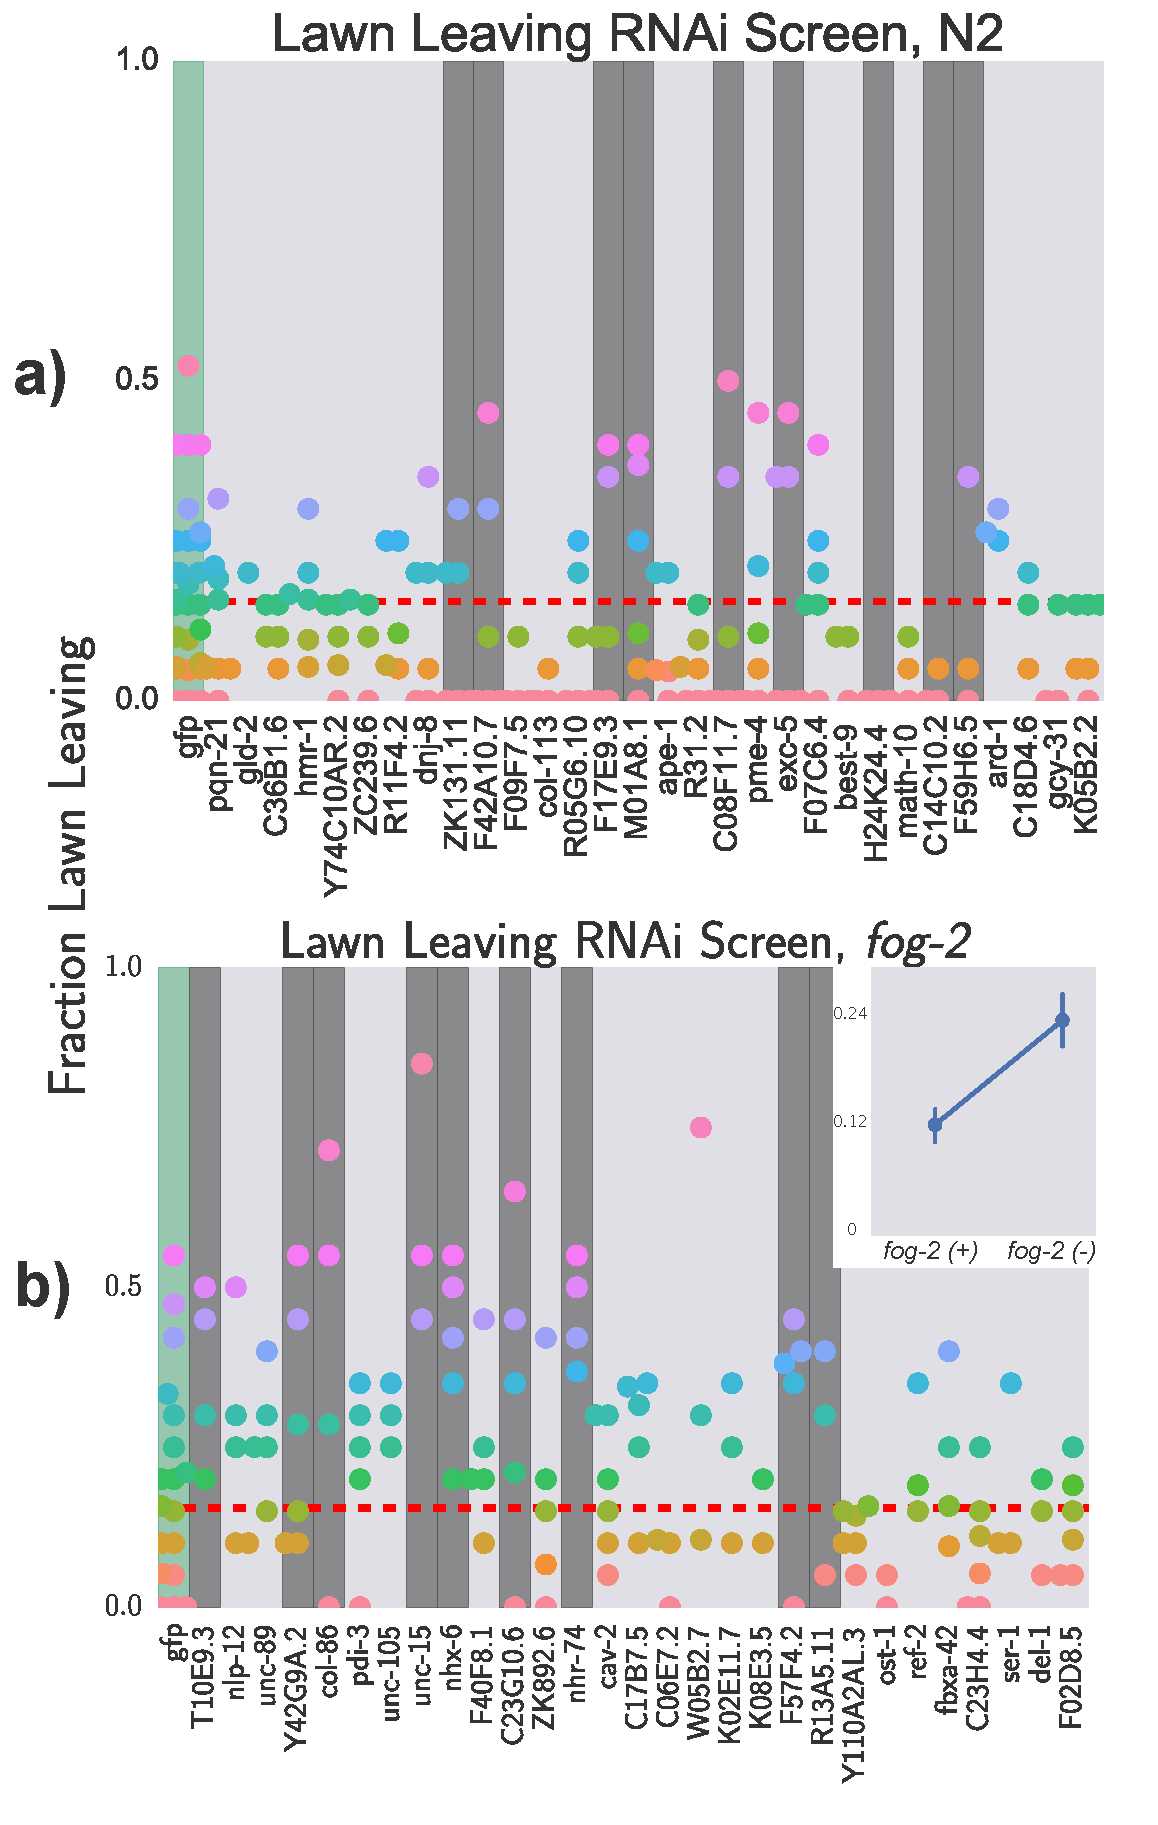
\includegraphics[width=\linewidth]{../output/figs/final_figs/lawn_leaving_rnai_assay.pdf}
\caption{lawn-leaving Screen Results. GFP control RNAi is shaded in green. Results that are statistically significantly different from GFP are shaded in dark grey. Dotted red line shows the mean of the pooled GFP controls. Points are colored proportionally to their y-coordinate. \textbf{a} N2 lawn-leaving assay. \textbf{b} \fog{} lawn-leaving assay. Inset shows the screen-wide average lawn-leaving rate of N2 and \fog{}, which shows that the screen-wide lawn-leaving rate of \fog{} worms is twice the rate of lawn-leaving of N2 worms, in agreement with previous literature~\citep{}.
}%
\label{fig:lawnleaving}
\end{figure}

We also performed lawn-leaving assays because previous research has reported differences in N2 and \fog{} leaving rates~\citep{}. We tested genes that increased in \fog{} animals in a \fog{} background, expecting that decreasing these genes should lead to a reversal of the lawn-leaving assay. Likewise, we tested genes that were decreased in \fog{} animals in an N2 background, expecting that knockdown of these genes would cause lawn-leaving. We identified 9 genes that had an altered lawn-leaving profile in an N2 background.
We also identified 9 genes that had an altered lawn-leaving profile in a \fog{} background. Oddly, both screens identified  genes that mainly stimulate lawn-leaving. Initially, we had expected that RNAi knockdown would allow us to identify genes that inhibit lawn-leaving behaviour in an N2 background; whereas RNAi knockdown in a \fog{} background would identify genes that promote lawn-leaving. However, our screen only identified genes that suppress lawn-leaving in an N2 background. All other hits stimulated lawn-leaving.

% n2
% ZK131.11 - pathogen defense
% F42A10.7 - stress
% F17E9.3 - nan
% M01A8.1 - fat content
% C08F11.7 - nan
% exc-5 - lethal, dev variant, locomotion variant
% H24K24.4 - tRNA methyltransferase
% C14C10.2 - locomotion
% F59H6.5 - dna helicase, dauer


% fog2
% T10E9.3 - nan
% Y42G9A.2 - nan
% col-86 -cuticle
% unc-15 - egl
% nhx-6 - ion channel
% C23G10.6 - enzyme
% nhr-74 - tf
% F57F4.2 - nan
% R13A5.11 - involved in reproduction



\section*{Discussion}
\label{sec:discussion}

\subsection*{Defining an Early Aging Phenotype}
\label{sub:Defining an Early Aging Phenotype}

Our experimental design enables us to decouple the effects of egg-laying from aging. As a result of this, we identified a set of almost 4,000 genes that are altered similarly between wild-type and \fog{} mutants. Due to the read depth of our transcriptomic data (20 million reads) and the number of samples measured (3 biological replicates for 4 different life stages/genotypes), this dataset constitutes a high-quality description of the genetic changes that occur in natural \cel{} aging.

\subsection*{Developmental Factors Change During Early Aging}
\label{sub:development_in_aging}

Our transcriptomic explorations revealed a host of transcription factors that changed during early aging in \cel{}. Many of these transcription factors have been associated with embryonic development via cellular differentiation and specification. For example, we identified the transcription factor \emph{lin-32}, which has been associated with neuron development~\citep{}; the Six5 ortholog \emph{unc-39} has been associated with axonal pathfinding; \emph{cnd-1}, a homolog  of the vertebrate NeuroD transcription factors, is expressed in the early embryo and its expression is reported to disappear by the end of the first larval stage~\citep{}.

Our explorations shown that the loss of the \fog{} transcription factor phenocopies early aging in \cel{}. The reason for phenocopying is unclear at this point, but we speculate that such a result could happen if an animal could sense its own fertilization status. Indeed, prior work has established that \cel{} is capable of detecting its fertilization state, and that this state has consequences for pheromone production and mating behaviours.
Given the enrichment of neuronal transcription factors that are associated with sperm loss in our dataset, we believe this dataset should contain some of the transcriptomic modules that are involved in these pheromone and behavioural pathways. Currently, we cannot judge how many of the changes induced by loss of hermaphroditic sperm are developmental (i.e., irreversible), and how many can be rescued by mating to a male. While an entertaining thought experiment, establishing whether these transcriptomic changes can be rescued by males is a daunting experimental task, given that the timescales for robust, whole-animal transcriptomic changes could reasonably be the same as the timescale of onset of embryonic transcription.

\subsection*{Interpretation of Screen Hits}
\label{sub:Interpretation of Screen Hits}





% \bibliography{example-bibliography}

\end{document}
